% !TEX root = ../my-thesis.tex
%
\chapter{PLANIFICACIÓN Y PRESUPUESTO}
\label{sec:planificacionypresupuesto}

En este capítulo se desarrollará la planificación llevada durante la elaboración del trabajo, con la que se ha conseguido superar cada uno de los objetivos marcados de forma satisfactoria. Además, se realizará un presupuesto orientativo del coste final que tendría el desarrollo de este trabajo.

\section{Planificación}

En primer lugar, para la facilidad de la gestión de las tareas y de los tiempos, se ha desglosado el trabajo en una Estructura de Descomposición del Proyecto (EDP). Esta división del trabajo total en tareas manejables, jerarquizándolas en forma de árbol.

Este EDP, se encuentra reflejado en la Figura \ref{fig:edp}, en forma esquemática, de manera que este queda dividido el trabajo en los siguientes 5 niveles:

\begin{itemize}
    \item \textbf{Aprendizaje:} Esto abarcan todas las tareas que han sido necesarias para la compresión adecuada de la temática del trabajo como cursos, lecturas o ejercicios.
    
    \item \textbf{Investigación:} Se compone de las tareas imprescindibles para la comprensión del estado actual de las diferentes tecnologías y desarrollos que se han estudiado durante la elaboración del trabajo.
    
    \item \textbf{Implementación:} Comprende todo el trabajo de realización de diseño y escritura del algoritmo que finalmente podrá ser ejecutado para comprobar los resultados buscados en este trabajo. 
    
    \item \textbf{Experimentación:} Se enumeran todos los experimentos que han sido necesarios realizar para la obtención de los resultados que se andaban buscando.
    
    \item \textbf{Elaboración del documento:} Se desarrolla este documento de forma escrita de manera que se sinteticen los aprendizajes y trabajos realizados.
    
\end{itemize}

\begin{figure}[!h]
    \centering
    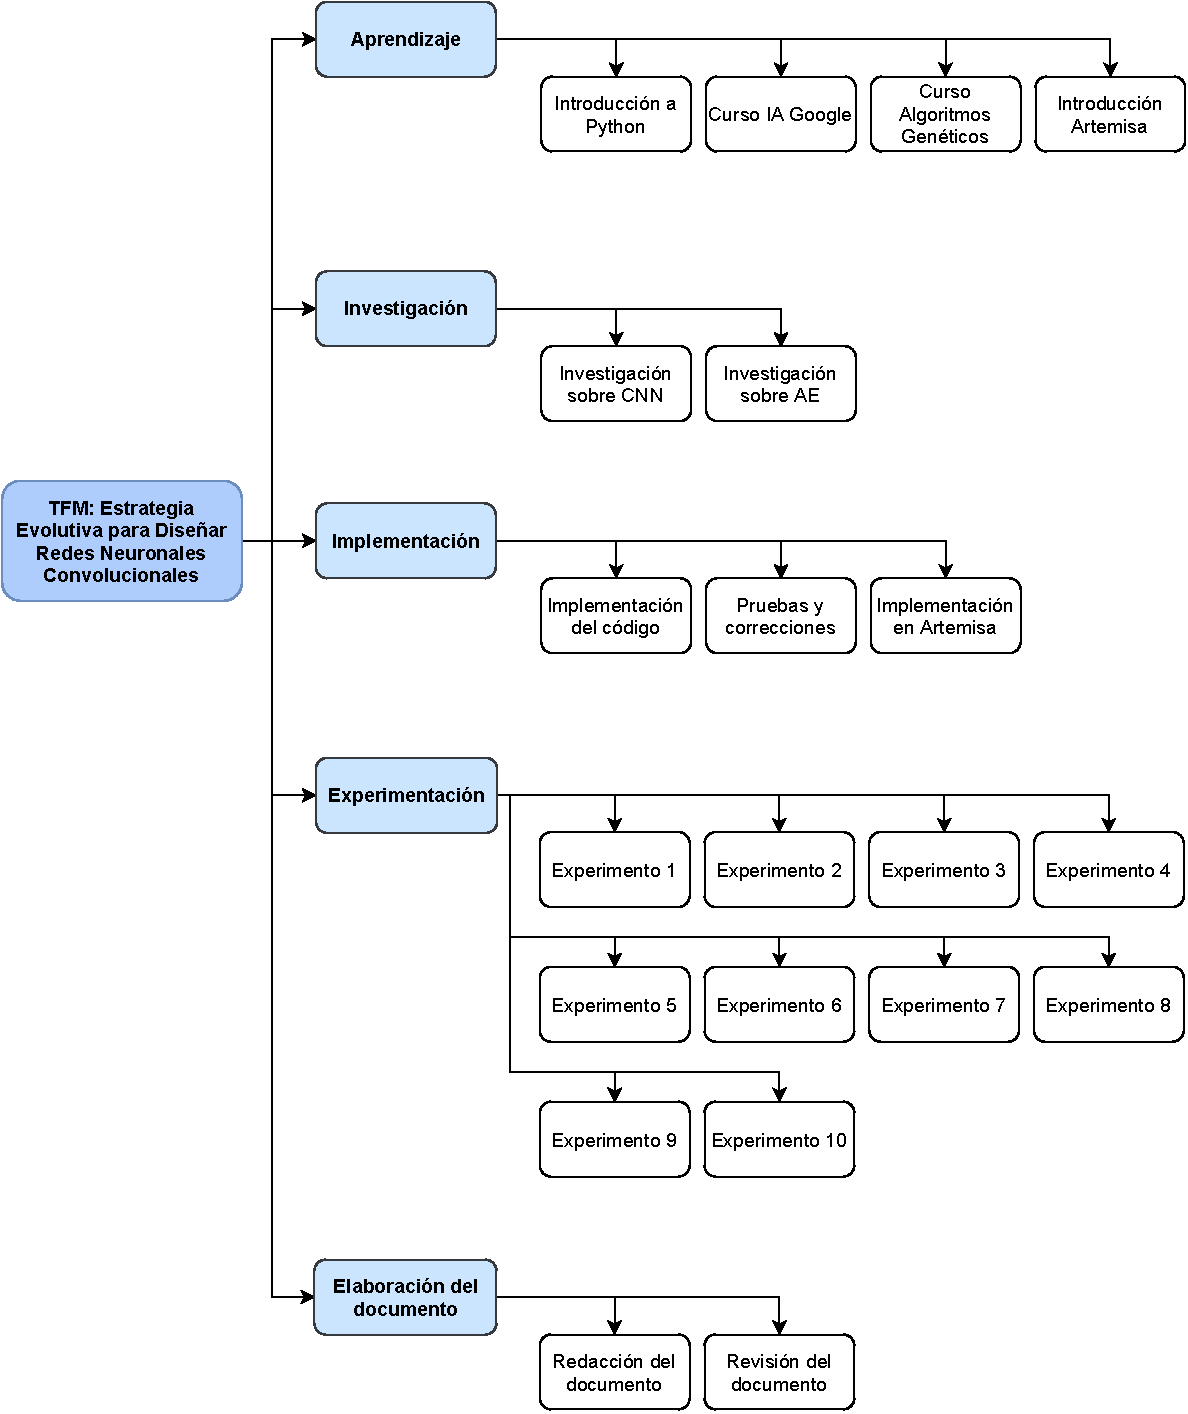
\includegraphics[width=\textwidth]{figuras/planificacion/EDP.pdf}
    \caption{EDP del trabajo}
    \label{fig:edp}
\end{figure}


Posteriormente, a cada una de estas tareas se les ha asignado una fecha de inicio y una fecha de final, de manera que se establezcan de forma temporal la dedicación a cada uno de los paquetes del EDP. Esto se ve reflejado en la Tabla \ref{tab:tiempos_planificacion}.


\begin{table}[!h]
\caption{Planificación temporal de las actividades necesarias para la elaboración del trabajo}
\label{tab:tiempos_planificacion}
\centering
\begin{tabular}{lll}
\toprule
\multicolumn{1}{l|}{\multirow{2}{*}{\textbf{Actividad}}}           & \multicolumn{1}{l|}{\multirow{2}{*}{\textbf{Fecha de inicio}}} & \multirow{2}{*}{\textbf{Fecha final}} \\
\multicolumn{1}{l|}{}                                              & \multicolumn{1}{l|}{}                                         &                                       \\ \hline
\multicolumn{3}{l}{\textit{Aprendizaje}}                                                                                                                                            \\ \hline
\multicolumn{1}{l|}{- Introducción a Python}                       & \multicolumn{1}{l|}{01/02/2021}                               & 26/02/2021                            \\
\multicolumn{1}{l|}{- Curso IA Google}                             & \multicolumn{1}{l|}{05/02/2021}                               & 12/02/2021                            \\
\multicolumn{1}{l|}{- Curso de Algoritmos Genéticos}               & \multicolumn{1}{l|}{15/02/2021}                               & 18/02/2021                            \\
\multicolumn{1}{l|}{- Introducción a Artemisa} & \multicolumn{1}{l|}{19/02/2021}                               & 26/02/2021                            \\ \hline
\multicolumn{3}{l}{\textit{Investigación}}                                                                                                                                          \\ \hline
\multicolumn{1}{l|}{- Investigación sobre CNN}                     & \multicolumn{1}{l|}{01/03/2021}                               & 14/05/2021                            \\
\multicolumn{1}{l|}{- Investigación sobre AE}                      & \multicolumn{1}{l|}{01/03/2021}                               & 28/04/2021                            \\ \hline
\multicolumn{3}{l}{\textit{Implementación}}                                                                                                                                         \\ \hline
\multicolumn{1}{l|}{- Implementación del código}                   & \multicolumn{1}{l|}{01/03/2021}                               & 20/05/2021                            \\
\multicolumn{1}{l|}{- Pruebas y correcciones}                      & \multicolumn{1}{l|}{03/03/2021}                               & 21/05/2021                            \\
\multicolumn{1}{l|}{- Implementación en Artemisa}                  & \multicolumn{1}{l|}{08/03/2021}                               & 19/03/2021                            \\ \hline
\multicolumn{3}{l}{\textit{Experimentación}}                                                                                                                                        \\ \hline
\multicolumn{1}{l|}{- Experimento 1}                               & \multicolumn{1}{l|}{22/03/2021}                               & 26/03/2021                            \\
\multicolumn{1}{l|}{- Experimento 2}                               & \multicolumn{1}{l|}{29/03/2021}                               & 02/04/2021                            \\
\multicolumn{1}{l|}{- Experimento 3}                               & \multicolumn{1}{l|}{05/04/2021}                               & 09/04/2021                            \\
\multicolumn{1}{l|}{- Experimento 4}                               & \multicolumn{1}{l|}{12/04/2021}                               & 28/04/2021                            \\
\multicolumn{1}{l|}{- Experimento 5}                               & \multicolumn{1}{l|}{19/04/2021}                               & 23/04/2021                            \\
\multicolumn{1}{l|}{- Experimento 6}                               & \multicolumn{1}{l|}{26/04/2021}                               & 07/05/2021                            \\
\multicolumn{1}{l|}{- Experimento 7}                               & \multicolumn{1}{l|}{26/04/2021}                               & 07/05/2021                            \\
\multicolumn{1}{l|}{- Experimento 8}                               & \multicolumn{1}{l|}{10/05/2021}                               & 14/05/2021                            \\
\multicolumn{1}{l|}{- Experimento 9}                               & \multicolumn{1}{l|}{17/05/2021}                               & 14/06/2021                            \\
\multicolumn{1}{l|}{- Experimento 10}                              & \multicolumn{1}{l|}{04/06/2021}                               & 17/06/2021                            \\ \hline
\multicolumn{1}{l|}{\textit{Elaboración del documento}}                     & \multicolumn{1}{l|}{}                                         &                                       \\ \hline
\multicolumn{1}{l|}{- Redacción del documento}                     & \multicolumn{1}{l|}{03/05/2021}                               & 17/06/2021                            \\
\multicolumn{1}{l|}{- Revisión del documento}                      & \multicolumn{1}{l|}{08/06/2021}                               & 28/06/2021   \\
\bottomrule
\end{tabular}
\end{table}

Finalmente con esta información, se puede mostrar de forma gráfica, apoyándose en un diagrama de Gantt como el que se puede observar en la Figura \ref{fig:gantt}, donde se ve de manera más visual la duración de cada una de las actividades.

\begin{figure}[!h]
    \centering
    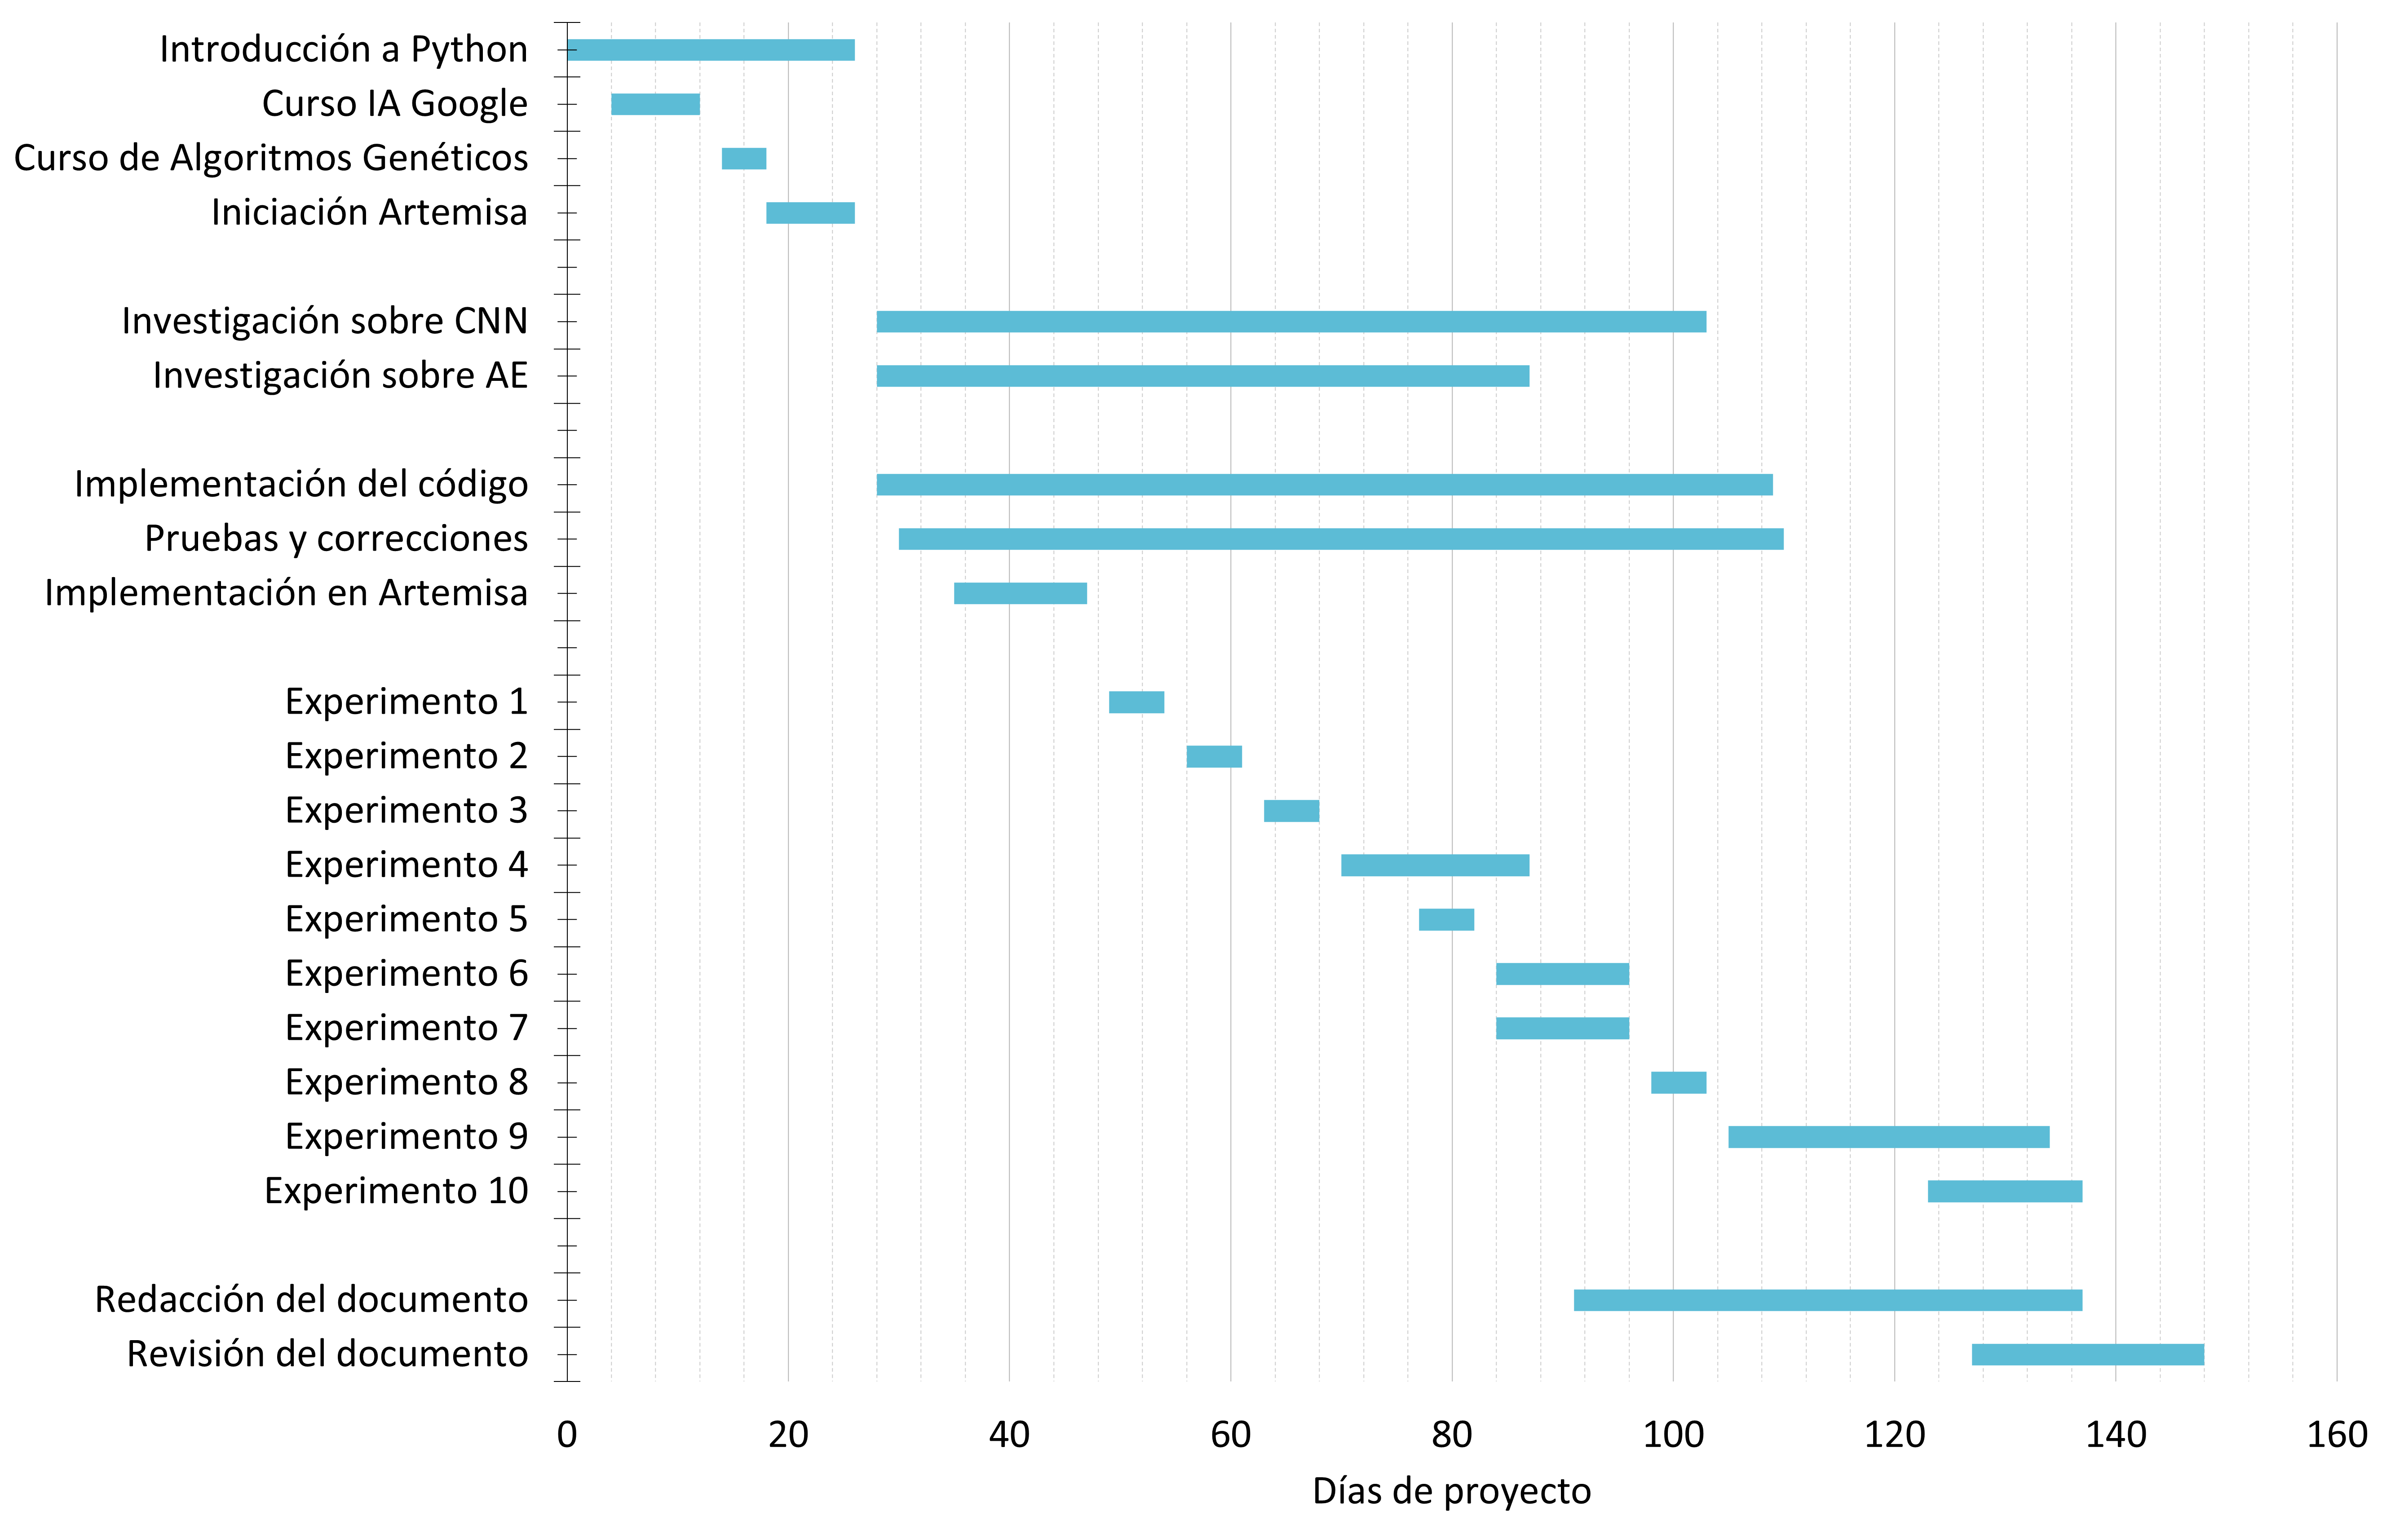
\includegraphics[width=1\textwidth]{figuras/planificacion/gantt.png}
    \caption{Diagrama de Gantt de la planificación temporal del trabajo}
    \label{fig:gantt}
\end{figure}


\section{Presupuesto}

Para la realización de este trabajo, han sido necesarios recursos materiales y humanos, que han de ser presupuestados para conocer el coste de la realización de este trabajo.

En primer lugar, haciendo alusión a los costes basados en los recursos humanos, se deben tener en cuenta las personas que han trabajado en sacar adelante este trabajo. Esto se compone de básicamente 3 personas, las cuales se dividen en los roles de la tutorización del trabajo, las del doctorando para la resolución de dudas y finalmente, del estudiante que ha realizado este trabajo.

Para el cálculo de horas de dedicación, se ha hecho unas aproximación basándose en las horas de dedicación establecidas por el estudiante a través de los créditos ECTS, pudiéndose ser mucho mayores las horas totales de dedicación por cada una de estas personas. En la Tabla \ref{tab:costes_humanos}, se puede ver a cuanto ascendería el total de estos costes, los cuales hacen un total de \textbf{10800 €}.

\begin{table}[h]
\caption{Costes de los recursos humanos involucrados en el trabajo}
\label{tab:costes_humanos}
\centering
\begin{tabular}{l|r|r|r}
\toprule
\textbf{Personal} & \multicolumn{1}{l|}{\textbf{Horas}} & \multicolumn{1}{l|}{\textbf{€/hora}} & \multicolumn{1}{l}{\textbf{Total (€)}} \\ \hline
Tutora            & 45                                  & 40                                   & 1800                                   \\
Doctorando        & 100                                 & 30                                   & 3000                                   \\
Estudiante        & 300                                 & 20                                   & 6000                                   \\ \hline
\multicolumn{3}{r|}{\textbf{TOTAL}}                                                            & \textbf{10800} \\
\bottomrule
\end{tabular}
\end{table}

Posteriormente, atendiendo a los costes materiales, este proyecto se basa en un desarrollo software, por lo que los gastos principales se basan en la amortización y alquiler de infraestructuras de computación y licencias de software. 

Para este primero, se ha calculado un valor aproximado del valor más significativo, que es el del uso de la infraestructura Artemisa, que tomando el valor de una infraestructura similar en la plataforma Azure de Microsoft, se establece que su coste mensual es de 600 € al mes, amortizándose al 100\%, durante un total de 5 meses. 

Por otro lado, se establece que el coste en licencias tales como el paquete de Microsoft Office, la licencia de Overleaf, el pack de desarrollo en Python de JetBrains y la licencia para el uso repositorios privados de GitHub, asciende aproximadamente a los 300 euros, amortizándose su total al 50\%.

En la Tabla \ref{tab:costes_materiales}, se pueden ver desglosados estos gastos, que ascienden a un total de \textbf{3290 €}.

\begin{table}[h]
\caption{Costes materiales del trabajo}
\label{tab:costes_materiales}
\centering
\begin{tabular}{l|r|r|r|r}
\toprule
\textbf{Concepto}     & \multicolumn{1}{l|}{\textbf{Coste Unitario (€)}} & \multicolumn{1}{l|}{\textbf{Unidades}} & \multicolumn{1}{l|}{\textbf{Total (€)}} & \multicolumn{1}{l}{\textbf{Amortizado (€)}} \\ \hline
Ordenador personal    & 700                                              & 1                                      & 700                                     & 140                                         \\
Licencias de software & 300                                              & 1                                      & 300                                     & 150                                         \\
Acceso a Artemisa     & 600                                              & 5                                      & 3000                                    & 3000                                        \\ \hline
\multicolumn{4}{r|}{\textbf{TOTAL AMORTIZADO}}                                                                                                              & \textbf{3290}  \\
\bottomrule
\end{tabular}
\end{table}

Finalmente, se puede extraer que el coste total de la elaboración de este trabajo, como se desglosa en la Tabla \ref{tab:costes_totales}, es de \textbf{14090€}.

\begin{table}[h]
\caption{Costes totales del trabajo}
\label{tab:costes_totales}
\centering
\begin{tabular}{l|r}
\toprule
\textbf{Concepto}                   & \multicolumn{1}{l}{\textbf{Total (€)}} \\ \hline
Costes Humanos                      & 10800                                   \\
Costes Materiales                   & 3290                                   \\ \hline
\multicolumn{1}{r|}{\textbf{TOTAL}} & \textbf{14090}  \\
\bottomrule
\end{tabular}
\end{table}